\section{Introduction}

Data-driven methodologies are currently revolutionizing how we model, predict, and control complex systems such as climate \parencite{knusel2020understanding}, finance \parencite{hilpisch2018python}, traffic \parencite{lin2018efficient}, robotics and autonomy \parencite{zhang2018review}. The most pressing scientific and engineering tasks of the present era are not dependent on empirical models or derivations based on first principles \parencite{brunton2019data}. Increasingly, researchers are turning to data-driven approaches for characterizing and modeling a diverse range of complex systems with the goal of sensing, prediction, estimation, and control. With modern mathematical methods, enabled by the unprecedented availability of data and computational resources, we are now able to tackle previously unattainable challenge. One such challenge is to analyze the performance of the electric machine in a relatively short period of time. An electromagnetic model is needed to perform the design and analysis of an electric machine \parencite{mousavi2015design}. This model will be used to evaluate relevant electromagnetic performance characteristics associated with an electric machine such as electromagnetic force, torque, fields, and losses distribution maps. Further, a model capable of providing an accurate and fast performance evaluation is the backbone of an optimization task for achieving objectives such as minimizing the torque ripple, increasing average torque and efficiency. It also plays a central role in designing the motor drive system. 

The very word `model' implies simplification and idealization. A model is an approximation of reality and hence will not reflect all of reality. 
In 1976, a renowned British statistician named George Box wrote the famous line, ``All models are wrong, some are useful" \parencite{box1979all, george_stat_eng}. The intuition behind this sentence is that every model is wrong because it is a simplification of reality. However, simplifications of reality can be quite useful. They can help us explain, predict and understand the universe and all its various components. It means useful insights can be provided from models which are not a perfect representation of the phenomena they model. The practical question is how wrong do they have to be in order to be not useful. As such, the desirable features of a model can be summarized as follows \parencite{silva2018}:

\begin{itemize}
    \item A model should be consistent in its ability to explain past observations and predict future observations.
    \item Cost of usage: A model should be computationally cheaper than traditional methods available for analysis. 
    \item Level of accuracy in the prediction: A model that gives highly accurate results but takes a lot of computational time may not be useful. On the other hand, a model that is not as accurate but can produce estimates very quickly can be beneficial.
\end{itemize}

% Intro-1
Maxwell's equations form the foundation of classical electromagnetism, classical optics, and electric circuits. We can consider models built on solving physics (such as Maxwell's equations) as the First Principle models \parencite{silva2018}. Modeling is the mathematical representation of physical phenomenona and simulation is the numerical representation of such models on computing machines. Over the years Computer-Aided Design (CAD) has evolved as the field of ``using computers to aid in the creation, modification, analysis, or optimization of a design" \parencite{sarcar2008computer}. 
Accurate modeling and analysis of an electromagnetic problem is both a challenging and time-consuming process due to several reasons.
First of all, the system of differential equations for the electromagnetic analysis of electric devices is nonlinear due to the property of saturation in magnetic materials. 
The non-linear dependence of inductances on rotor-to-stator angles is reflected in the non-linear relationship between current and fluxes. Since the induced voltage and electromagnetic torque are proportional to the state variables, such as flux, current, and speed, it makes it impossible to find an analytic solution to the machine system of differential equations \parencite{ostovic2012dynamics}. If we neglect the effects of saturation and non-linear magnetic materials, a model will be suitable for only a fraction of a device's operating capacity. Apart from the difficulty of solving a nonlinear system of equations, finding a field solution on a complex geometry such as that of an electric machine also adds to the complexity of the task.

% Intro-5
Having identified the challenges associated with the field of electromagnetic modeling and simulation, we can broadly divide the field into three categories of algorithms namely: Analytical, Numerical, and Magnetic Equivalent Circuits (MEC), as shown in Figure \ref{fig:CNN_model_techniques}. Of the three, analytical algorithms are usually the least demanding in terms of computational need and will provide the fastest results. These methods try to find the closed-form expressions for magnetic fields and losses in a motor. However, they face a major challenge in approximating complex geometries and incorporating the effect of iron saturation in their analysis \parencite{alger1970induction,hamdi1994design}, which is significant for estimating magnetic fields and losses of the motors \parencite{sheikh2009improved}. Furthermore, they are incapable of modeling skin and proximity effects in the winding and the end winding inductance. Despite their limited capabilities, analytic models are popular because of the low computation power required for their highly simplified expressions and ease of parameterization. As a result, they are employed when fast prototyping is needed and the design is evaluated only on the basis of global performance quantities such as torque and forces \parencite{ray1984switched, krishnan1988design}.

\begin{figure}
    \centering
    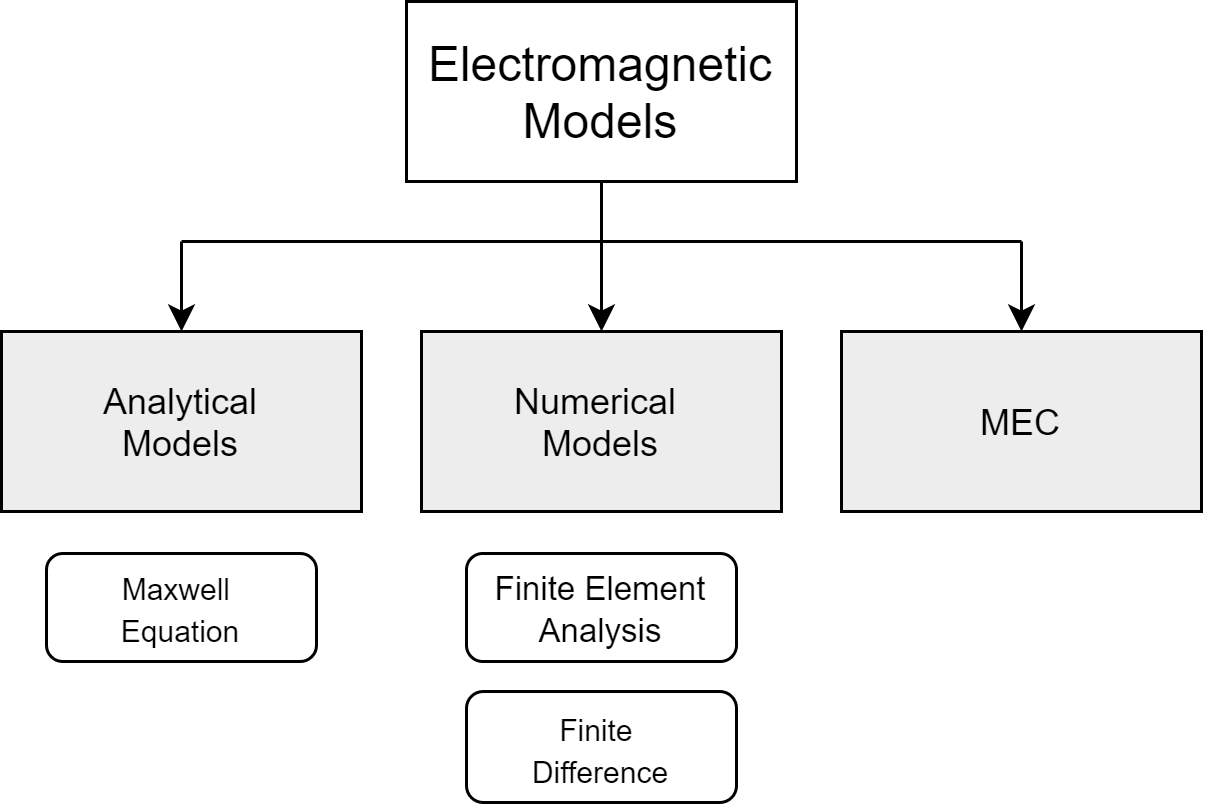
\includegraphics[width=0.65\textwidth]{Figures/Chp2_CNN/EM_model_techniques.png}
    \caption{Different electromagnetic modeling techniques.}
    \label{fig:CNN_model_techniques}
\end{figure}

% Intro-6
The physics-based models, on the other hand, are founded on established and detailed physical principles and lead to more accurate simulations \parencite{salon1995finite}. They model the interaction of electromagnetic fields with physical objects and the environment. Two such methods are Magnetic Equivalent Circuits (MEC) and Finite Element Analysis (FEA). 

% Intro-7
The MEC modeling is a popular method in modeling electric machines \parencite{yilmaz2008capabilities}. It is a special case since it can be considered as an analytical or numerical technique according to how it is applied. It is considered as an analytical technique if it is combined with other analytical modeling techniques such as Maxwell’s equations \parencite{uddin2017analytical, radun2000analytically}. When the nonlinearity of the magnetic materials is considered, the MEC modeling has to be combined with numerical techniques \parencite{ostovic2012dynamics}. In \cite{ostovic2012dynamics}, the MEC method was applied to calculate the magnetic flux in C-core magnetic devices and also to model magnetic devices with moving parts such as electric machines.

The present-day Finite Element (FE) method based software suite allows for the accurate analysis of electric machines in three dimensions with coupled fields. It is the method of choice for today's machine designers, in comparison to analytical models and MECs. Finite Difference Methods (FDM) are another option to model electric machines. However, FDM has difficulties in modeling complex geometries; therefore, it is not directly applied to model electric machines \parencite{hameyer1999numerical}.

% Intro-8
Another class of models, surrogate or data-driven models, is not necessarily based on first principles. They approximate the relationship between the input parameters and output characteristics and reduce the repetitive bottom-up approach taken by the first principle models. Machine Learning (ML) and curve-fitting-based techniques are some of the approaches in this category of modeling used to predict the performance of electric machines. 
They include experimental or Finite Element (FE) model data to develop the model. These methods can provide a fast prediction of global performance parameters such as average and ripple torque \parencite{mohammadi2019data, ibrahim2020surrogate}. 
However, these models, based on current the literature, are not capable of producing information on local effects within the device such as fields, losses, and stresses. Knowledge of the flux distribution inside the motor for different operating conditions is essential, at the design stage, to predict the performance \parencite{watthewaduge2020electromagnetic}. The saturation and the geometry of the motor structure make the analytical methods of field analysis difficult. This chapter will explore the field of Deep Learning (a sub-field of ML) to predict the field distribution for different electromagnetic problems. Since ML models require labeled data for training and without an accurate model, it is impossible to predict a machine's characteristics and performance. As such it is important to identify a reliable source to generate training data for the ML task. Since analytical models are not capable of capturing sufficient information for the analysis of electric machines, the discussion will be limited to only MEC and FEA, to serve as the source of data generation. 

\begin{comment}
Whereas, motor losses arising from flux density distribution are already accounted for in FEA solution \parencite{haisen2013effective}.

% Intro-4
Electric Machine models can be broadly categorized into the lumped parameter and physics-based models. Lumped parameter models, such as phase-domain (PD) and direct-quadrature (d-q) models, have been heavily studied over the last half-century \parencite{wang2007re}. Lumped Parameter (LP) models can calculate only a few metrics such as average torque \parencite{lovelace2002saturating}, with additional information like torque ripple and iron loss lost.  Overall, such models are suitable for studying small changes to established designs, but they fall short when considering radical designs or seeking more accurate representations. 

\textit{ } \parencite{amrhein2007magnetic}

\textit{Although some researchers have presented methods to consider motion in PM motors, the change of reluctance network during motion adds to the complexity of solving equations [37], [38], [15].}
\end{comment}


\section{Physics-based Modeling}

Before finalizing the source of labeled data, it is important to understand the capabilities and limitations of FE analysis and MEC in reference to electric machine design analysis. Based on the study, we will determine the numerical method suitable to generate the synthetic training data. The literature on FE and MEC based techniques is vast and covers the analysis of a variety of electric devices. This study is limited to only electric machines, as they are the primary motivation of this work.

\subsection{Finite Element Methods}

The FE method is applied to design and analyze electric motors and generators with various stator/rotor topologies \parencite{mousavi2015design, rosu2017multiphysics}.
It is a numerical model for solving problems of engineering and mathematical physics by formulating the problem results in a system of algebraic equations. FE analysis can be broken down into four broad steps \parencite{jin2015finite, salon1995finite}:
\begin{itemize}
    \item Domain Discretization.
    \item Selection of Interpolation Functions.
    \item Formulation of the System of Equations.
    \item Solution of the System of Equations.
\end{itemize} 

A proper discretization optimizes the number of elements and unknowns for the desired solution accuracy because the manner in which the domain of the solution is discretized will affect the memory storage space, computation time, and the accuracy of the numerical solution. 

The process of generating a system of equations is to convert a continuous operator problem to a discrete problem. This step is more involved and depends on the specific FEM method used (two popular methods are Ritz and Galerkin \parencite{silvester1996finite}). The whole cycle of the FEM model can be shown in Figure \ref{fig:FEM}.

\begin{figure}[h!]
\centering
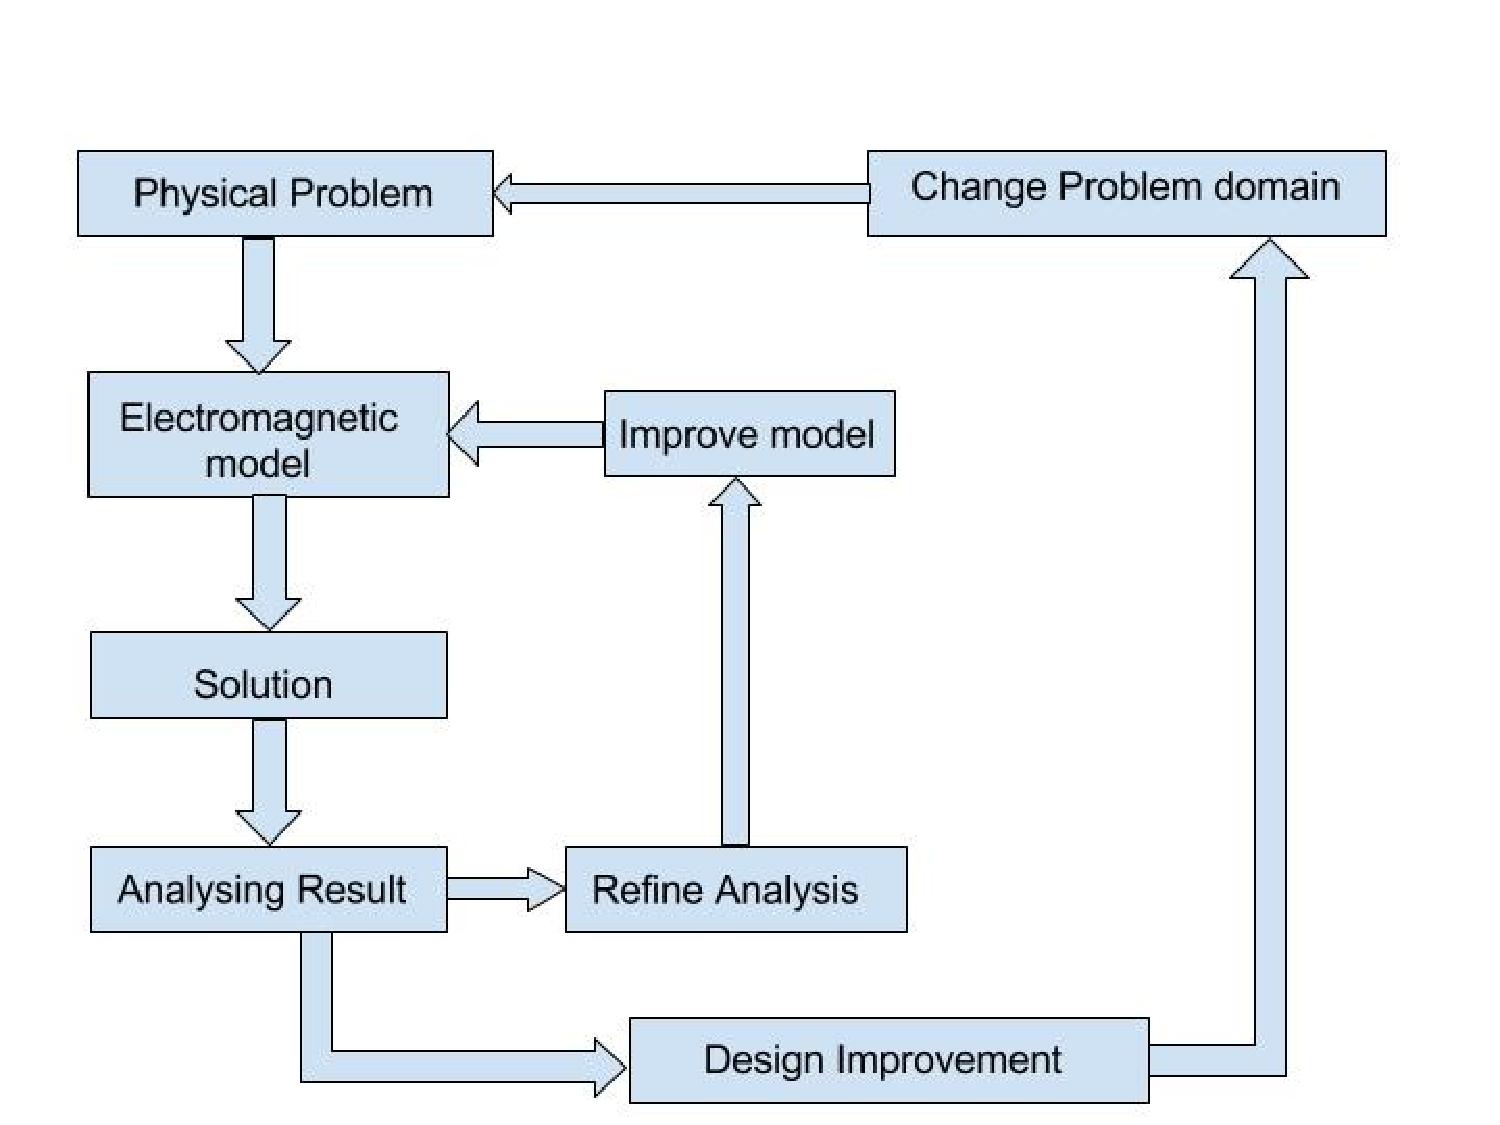
\includegraphics[width=0.85\textwidth]{Figures/Chp2_CNN/Proposal.pdf}
\caption{Computational Analysis in FEM}
\label{fig:FEM}
\end{figure}

% 8C
The final accuracy of the results reported in a finite element analysis model depends on many factors. One of the primary factors for accuracy is the number of mesh elements \parencite{bianchi1998design}. It is necessary to increase the number of elements in the highly saturated regions to improve the model accuracy. Among all numerical modeling techniques, FE is considered the most popular technique for modeling machines that operate in magnetic saturation conditions \parencite{bostanci2017opportunities}. Moreover, since the machine airgap is changing with the rotation of the rotor, it will also require a large number of elements.

The field solution can be obtained using various numerical methods, for example, LU Decomposition, Banded Choleski, the Conjugate Gradient Method, and the Preconditioned Conjugate Gradient Method. These methods work by reducing the error between an estimate and the unknown solution at every iteration.
% 8F
Due to the nonlinearity of the magnetic materials, the formulated system of equations is nonlinear. The Newton-Raphson method is used to solve the system of equations \parencite{salon1995finite}. For electric motors, post-processing is afterward applied to the converged magnetic vector potentials to calculate various electromagnetic quantities such as flux linkage, flux density, and electromagnetic torque.

% SRM Modeling, Design, Simulation and Analysis

\begin{comment}
An understanding of the improvements to be gained in energy conversion efficiency through exploitation of magnetic saturation.

Difference between Linear and NL methods?

\end{comment}

\subsection{Magnetic Equivalent Circuits}

MEC models, in general, are seen as a compromise between FEM and lumped parameter models \parencite{sudhoff2007magnetic}. They take machine geometry and material characteristics into account and are thus more refined than lumped parameter models \parencite{amrhein2007magnetic, moallem1998improved}. The circuit-oriented approach makes them a more intuitive design tool compared with FEM models \parencite{tavana2016real,asghari2012experimental}. 

MECs offer an alternative possibility that is based on permeance network models comprising reluctance and mmf sources. In general three types of elements appear in MEC: mmf sources, flux sources, and permeance. Node potential methods \parencite{osto1987} solve the MEC. The MEC can be considered as a reduced order FE which translates a geometrical description of a magnetic device consisting of coils of wire, a magnetic conductor such as iron, and permanent magnet material into an electrical circuit description \parencite{krause2013analysis}. By taking into account an approximately accurate machine geometry, stator, and rotor slots effects, skewing, the type of winding connections, stator and rotor leakages, and linear or nonlinear magnetic characteristics of machine cores it provides a comparatively more accurate solution than analytic methods \parencite{carpenter1968magnetic}. An electric machine is assumed to be a quasi-stationary device; that is, any change of current that builds the flux is followed by an immediate change of flux (In other words, the time needed for an electromagnetic wave to pass through the machine is negligible compared to the period of the wave). Such a space may be partitioned into flux tubes. The flux tubes are the basis of the magnetic equivalent circuit method. A flux tube is a geometrical space in which all lines of flux are perpendicular to their bases, and no lines of flux cut their sides \parencite{ostovic2012dynamics}. 

Currents flowing in the windings are the MMF sources in the magnetic equivalent circuit of an electric machine. These MMF sources are placed in the teeth. A reluctance/permeance and an unknown flux are assigned to each yoke part or each tooth. Slots are modeled by their leakage permeances. In the air gap, a flux tube is defined when any of the stator teeth come face to face with a rotor tooth. Permeance is assigned to each air-gap flux tube. Geometries of these flux tubes vary due to the rotation of rotor teeth with respect to stator teeth and also depend on the air-gap length between any two facing stator and rotor teeth. Any air-gap asymmetry will affect the height of these flux tubes. Although some researchers have presented methods to consider motion in motors, the change of reluctance network during motion adds to the complexity of solving equations \parencite{zhao2011survey, zhang2006finite}

\subsection{Comparison between MEC \& FEA}

The finer modeling and simulation resolution offered by FE analysis enables us to study complex issues such as internal faults or localized magnetic saturation in machines \parencite{wang2007re}. FEM models are computationally very intensive, and the model size and time step constraints make them unsuitable for use in a real-time simulation environment \parencite{tavana2016real,liu2009equivalent}. Hence in the case of limited computation capability, FEA models are used for final design analysis only. 
 
The advantages of the MEC method include reduced model complexity compared to FE, ease of parameterization, and fast computational time \parencite{yilmaz2008capabilities}. MEC has gained popularity in past years mainly since the extension to 3-D does not expand the numerical complexity as quickly as with FEA \parencite{kim2002analysis,amrhein2007magnetic}. MEC is also useful for performance analysis and initial device sizing. However, it may be inadequate for the accurate representation of complex geometric shapes and nonlinear material properties. A comparison of reported results between FEA and MEC simulations against experimental measurements is shown in Table \ref{table:2}. It can be observed that both FEA and MEC exhibit acceptable accuracy against experimental results.

\begin{table}[H]
\centering
\begin{tabular}{||c|c|c||}
\hline
\hline
\textbf{Ref} & \textbf{Method} & \textbf{Force/Torque Comparison}\\
\hline
\hline
\multirow{2}{*}{\parencite{liu2006closed}} & \multirow{2}{*}{FEA-MEC} & 6\% on force between MEC and test \\
 & & 10\% on force between FEA and test \\
\hline
\multirow{3}{*}{\parencite{hur1997analysis}} & \multirow{3}{*}{FEA-MEC} & 8.6\% on force between 2D MEC and test \\
& & 9\% on force between 2D FEA and test\\
& & 1\% on force between 3D MEC and test\\
\hline
\multirow{2}{*}{\parencite{leplat1996comparison}} & \multirow{2}{*}{FEA-MEC} & 16.9\% on torque between MEC and test\\
& & 11.1\% on torque between FEA and test\\
\hline
\multirow{2}{*}{\parencite{kim2004static}} & \multirow{2}{*}{FEA-MEC} & 3-5\% on force between FEA and test\\
& & 5-35\% on force between MEC and test\\
\hline
\end{tabular}
\caption{Experimental and Simulation result comparison}
\label{table:2}
\end{table}

FE analysis has both advantages and disadvantages relative to MEC based analysis. Regarding benefits, FEA generally requires less deployment time for simulation. The direction of flux in each element of the MEC model must be known before the MEC method is applied, whereas, in FEA, one of the results of computation is the flux distribution itself \parencite{ostovic2012dynamics}. In addition to that, FEA is generally more accurate than MEC analysis. FEA also offers a comparatively more flexible tool to study designs incorporating new shapes as compared to any other models discussed thus far. Based on this study, it is decided that FE offers the flexibility to model complex geometries and generates the field solution with high accuracy and thus is ideal for populating the training dataset consisting of thousands of simulated designs.

\subsection{Need for an Improved Surrogate Model}

Having discussed the advantages and limitations of the popular numerical methods associated with the analysis of electric machines, it is clear that a computationally cheap and accurate field solution is necessary for the analysis of electromagnetic devices such as actuators, transformers, and electrical machines \parencite{yilmaz2008capabilities, silva2018surrogate, silva2017surrogate}. This can be a challenging task and usually for generating an optimal design, we need to perform a few thousand analyses as part of optimization. Usually, once a handful of designs are shortlisted using MEC or d-q analysis, testing of these designs with 3-D FEA is performed. There have been studies where FEA is used for design step directly \parencite{bianchi1998design,salon1995finite}. However, this dramatically reduces the size of search space and is computationally very expensive due to longer analysis time.
Decades of research and engineering have gone into designing fast numerical solvers for design analysis. However, employing FE methods for modeling and simulation purposes remains a computationally expensive process and is still an active field of research. This has also led to the development of alternative surrogate models to accurately evaluate and/or optimize a device \parencite{silva2018surrogate, silva2017surrogate, wang2016neural, ghorbanian2017computer, ghorbanian2017statistical}. Unfortunately, these surrogate methods are usually specific to a problem and describe systems with very few parameters, thus limiting the ability of such surrogate models to deal with any arbitrary change in the design of a machine \parencite{silva2017surrogate}. On the other hand, in recent years, rapid developments in the field of machine learning (ML) and big data \parencite{krizhevsky2012imagenet}, have opened new venues for pattern recognition and curve fitting in complex problems such as computer vision \parencite{krizhevsky2012imagenet, he2016deep}, dense regression \parencite{badrinarayanan2015segnet}. Most of the recent work in this growing field of research is related to improving data-driven statistical methods to supplement simulations to solve engineering problems. These works are shown across applications such as smoke simulation \parencite{chu2017data}, liquid splash modeling \parencite{um2018liquid} and modeling liquid behavior with obstacles \parencite{tompson2017accelerating}. Another work, which is more related to this discussion, tried solving Poisson’s equation with a Deep Learning (DL) algorithm \parencite{tang2017study}. The use of deep networks suitable for the task for magnetic field estimation might accelerate the solution of such problems. Hence, the possibility of applying deep networks to magnetic field estimation is investigated in this work, for the domain of low-frequency EM devices, using a bitmap approach.

\section{Machine Learning}

Although DL has gained a lot of importance in recent times, it has been in existence since 1940. The first experiment with neural networks was performed in the 1940s \parencite{mcculloch1943logical} and the algorithms to train deep networks have been present since 1980. The first successful application of Convolutional Neural Networks(CNN/ ConvNets) was developed by Yann LeCun \parencite{lecun1998gradient} in the 1990s. The most popular of those architectures is known as \textit{LeNet}, which was used to read zip codes, handwritten digits, etc. Utilization of these concepts for producing state of the art results in more evolved fields such as computer vision \parencite{he2015delving}, text analysis \parencite{devlin2018bert}, forecasting, etc., demands computational memory and speed which was not available on mainframes until a few years back. At one point in time, this field was regarded as an art rather than a science due to the difficulty involved in successfully training these models, but that is not the case anymore. Some other reasons that have contributed to the success of these deep models today are the resources available both regarding training data and software libraries such as Tensorflow\parencite{tensorflow2015-whitepaper}, Theano \parencite{theano}, PyTorch \parencite{paszke2017automatic_pytorch}, etc. Also, these algorithms have undergone some major changes in the past decade which have greatly simplified the training process. 

Due to the advancement in computational technologies and improvement in DL algorithms\parencite{hinton2006fast, bengio2007scaling, delalleau2011shallow}, the number of hidden units in an artificial neural network has doubled in size every 2-3 years \parencite{goodfellow2016deep}, since the late 2000s. Some of the major factors that can be attributed to this growth are:

\begin{itemize}
    \item Computation Power (GPUs, ASICs, TPU (Tensor Processing Unit)).
    \item Data (Both ability to generate massive datasets and process them).
    \item Improvement in algorithms (CNN, LSTM (Long short term memory)).
    \item Infrastructure \& Frameworks (Git, Cloud Computing, Tensorflow \parencite{tensorflow2015-whitepaper}).
\end{itemize}

As for defining `Deep Networks', there is no universally agreed-upon threshold of depth dividing shallow learning from deep learning. One of the earliest deep neural networks had three densely connected hidden layers \parencite{hinton2006fast}. In 2014, VGG networks consisted of 16+ hidden layers and were called `Very Deep' networks \parencite{simonyan2014very}. In 2016 the ``Extremely Deep" residual networks \parencite{he2016deep} consisted of 50 to 1,000 hidden layers. For Feedforward Networks, CAP is the number of hidden layers plus one. Formally, CAP (Credit Assignment Path) is the chain of transformations from input to output. Most researchers in the field agree that deep learning has multiple nonlinear layers (CAP $\geq$ 3) and Schmidhuber \parencite{schmidhuber2015deep} considers CAP $\geq$ 10 to be very deep learning. So, a neural network with more than one hidden layer can be considered a Deep Network.

Why and where should one use a Deep Neural Network? As the number of features increases in our data, it becomes difficult to train a linear model. The interaction between these features can be too complicated for simpler models to achieve satisfactory accuracy. On the other hand, deep neural networks can adapt to more complex datasets and generalize to previously unseen data; thus they can fit more complex data than linear models can. It has been observed that the network’s performance degrades if a single layer is removed \parencite{krizhevsky2012imagenet}. However, the tradeoff of an additional layer is that the model will take longer to train, will be larger in size, and have lesser interpretability. One of the trickiest things about these networks is to get a configuration of parameters that works. There can be multiple possibilities of these configurations. 

The way the model is trained, i.e., the starting position, optimization algorithms, learning rate, etc., plays an essential role in the success and failure of our model. For the DL models trained in this chapter, the outcome/target/label/dependent variable is in the form of a quantitative quality (magnetic field distribution), which is predicted based on the information related to geometric features, excitations and the material properties, all of which will constitute the features/predictors/independent variable. Having identified the training data, the next step is to perform statistical learning that will enable us to predict the field solution of new unseen geometries. This type of learning is a case of supervised learning. The next few sections will dig deep into the complete ML pipeline. The first step (discussed in Section \ref{sec:CNN_DataCollection}) in the pipeline is the collection of training data in a format suitable for training a DNN. Once sufficient data is collected different neural network architecture are explored to suit the learning task, This process is discussed in Section \ref{sec:Arch_CNN}, followed by the working of the Neural network in Section \ref{sec:Work_CNN} and the decision-making process involved in tuning the network suitable for the task at hand. Results based on this pipeline are shown in Section \ref{sec:results_CNN}. 

In addition to magnetic field estimation, identifying when the input does not fit the problem description is also essential and is handled very well by an FEA solution system. Basically, a ML network trained in a supervised manner could predict the solution for any arbitrary input. As such, a DL emulator lacks a physics-based judgment. This is an important issue that will be addressed through an uncertainty analysis over the prediction, to generalize the DL estimator as much as possible.

\section{Data Collection} \label{sec:CNN_DataCollection}

Deep Learning models usually have many parameters to be tuned and therefore need a lot of data to generalize. The input data is called a dataset.
A `dataset' is defined as a collection of instances that share some common attributes. One of the most significant attributes related to a dataset is the type of task which is also referred to as the `target'. The other important attribute is the domain, which is the source of the data. The domain and task characterize a supervised learning problem.

In supervised learning, the two most important types of learning problems can be characterized based on the type of task, which are classification and regression. For a Classification task, the target is a label (also known as class) where the task is to match the samples with existing entities in the form of classes. On the other hand Regression is an example of supervised learning where the task is to predict a number by learning a function relating the input and output.

The performance of any ML algorithm is only as good as the data used to train it. A weak representation of the ML problem insufficiently captures the dynamics necessary to successfully learn the mapping of inputs to outputs. 

A weak representation of a problem can be attributed to two main reasons:

\begin{enumerate}
    \item Missing important information of the domain representation (input).
    
    \item The dataset, which is a sample of a population, does not represent the population in an unbiased manner. 
\end{enumerate}

To tackle the above issues, the input data is represented using the CAD geometry along with information related to the material distribution and excitations, at sufficient resolution. Further, all the samples are populated using a Latin Hypercube.

Depending on the complexity of the problem, different network architectures or parameters might be considered in the search for an optimal structure to guarantee a reasonable prediction error. Therefore, to appropriately establish the idea of DL for magnetic field estimation, three problems with different complexities of the geometry, material, and excitation, i.e. a simple coil in air, a transformer \parencite{Bottauscio} and an Interior Permanent Magnet (IPM) machine \parencite{wang2016neural, ghorbanian2017computer, ghorbanian2017statistical} are incorporated. All the three problems are parameterized and simulated in the FEA software package – MAGNET \parencite{Magnet}. All the materials properties including the non-linear (NL) nature of the B-H relation were used as is mentioned in the material library of MAGNET \parencite{Magnet}. 

Given the goal of this work, i.e. predicting the field distribution in electromagnetic devices using DL, a set of inputs and outputs used for training the networks must be generated first. The input of the network is formatted as a uniform structured grid containing information regarding the geometry, material, and excitation at each node in the input (pixel).

\subsection{Coil}

A simple coil made of copper is located inside an airbox, whose dimensions (height = 160mm, width = 160 mm) are fixed. However, the radius of the coil ($3mm \leq$ R $\leq 15mm$) as well as its center’s position change as the parameters of the problem. Constraints are placed to make sure the entire coil remains inside the box and that the radius is determined first and the center is adjusted accordingly. The coil current is also changed from 5A to 15A.

\begin{figure}[h!]
    \centering
    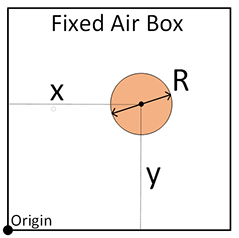
\includegraphics{Figures/Chp2_CNN/Geo_coil.png}
    \caption{Parametrized Geometry - Coil.}
    \label{fig:CNN_Fig-2_Geo_coil}
\end{figure}

\subsection{Transformer}
A transformer with two coils, one of which is not excited, is considered as the second problem which is more complex than the coil problem in terms of the geometry, material, and field distribution. The transformer core is made of M19 silicon steel material(NL). The coils are made up of copper, and the dimensions change as in Table \ref{tab:cnn_transformer_parameters}. The left coil’s current is fixed at 1A and there are 90 turns and the right coil’s current is zero. The transformer depth is 2.5mm.
\\
\\

\begin{minipage}{\textwidth}
  \begin{minipage}[b]{0.55\textwidth}
    \centering
    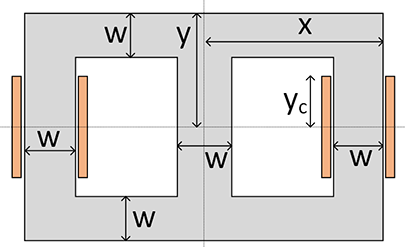
\includegraphics[width=\textwidth]{Figures/Chp2_CNN/Geo_Tf.png}
    \captionof{figure}{Parametrized Geometry-Transformer.}
    \label{fig:CNN_Fig-2_Geo_transformer}
  \end{minipage}
  \hfill
  \begin{minipage}[b]{0.4\textwidth}
    \centering
    \begin{tabular}{|c|c|c|}
        \hline 
        \textbf{\begin{tabular}[c]{@{}c@{}}Para-\\ meter\end{tabular}}
        & \textbf{\begin{tabular}[c]{@{}c@{}}Minimum\\ (mm)\end{tabular}} 
        & \textbf{\begin{tabular}[c]{@{}c@{}}Maximum\\ (mm)\end{tabular}} \\ 
        \hline \hline
        x     & 10 & 190 \\ \hline
        y     & 10 & 190 \\ \hline
        w     & 5  & 150 \\ \hline
        $y_c$ & 5  & 50  \\ \hline
        \end{tabular}
        \captionof{table}{Transformer Parameters}
        \label{tab:cnn_transformer_parameters}
    \end{minipage}
\end{minipage}

\subsection{IPM Motor}
A 4-Pole, 24-slot IPM motor is analyzed as the most complex problem in this work. In addition to M19, and copper, permanent magnets (NdFeBr) are also incorporated. Table \ref{tab:cnn_ipm_motor} lists the parameters of the IPM motor. The stator windings have 8 turns and the excitation current was varied from 25 A to 35 A rms. A partial (one pole) model is used for the simulations to reduce the computation time.

In addition to magnetic field estimation, identifying when the input does not fit the problem description is also essential and is handled very well by an FEA solution system. Basically, a ML network trained in a supervised manner could predict the solution for any arbitrary input. As such, a DL emulator lacks a physics-based judgment. This is an important issue that will be addressed employing the uncertainty analysis, to generalize the DL estimator as much as possible.

\begin{minipage}{\textwidth}
  \begin{minipage}[b]{0.35\textwidth}
    \centering
    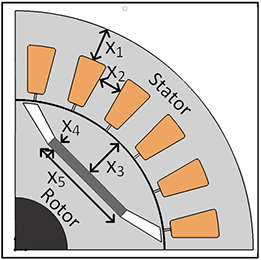
\includegraphics[width=\textwidth]{Figures/Chp2_CNN/Geo_motor.png}
    \captionof{figure}{Parametrized Geometry - IPM Motor.}
    \label{fig:CNN_Fig-2_Geo_motor}
  \end{minipage}
  \hfill
  \begin{minipage}[b]{0.6\textwidth}
    \centering
    \begin{tabular}{|c|c|c|}
        \hline
        \textbf{Parameter} 
        & \textbf{\begin{tabular}[c]{@{}c@{}}Minimum\\ (mm)\end{tabular}} 
        & \textbf{\begin{tabular}[c]{@{}c@{}}Maximum\\ (mm)\end{tabular}} 
        \\ \hline \hline
        Stator back iron ($x_1$)          & 5  & 35 \\ \hline
        Stator tooth width ($x_2$) & 5  & 12 \\ \hline
        Magnet inset depth ($x_3$) & 5  & 25 \\ \hline
        Magnet thickness ($x_4$)   & 1  & 50 \\ \hline
        Magnet width ($x_5$)       & 20 & 50 \\ \hline
        \end{tabular}
        \captionof{table}{IPM Motor Parameters}
        \label{tab:cnn_ipm_motor}
    \end{minipage}
\end{minipage}

\section{Neural Networks}\label{ANN}

%This is from CS 231 Stanford---include in bib

Neural Networks consist of collections of neurons that are connected in an acyclic graph. In other words, the outputs of the neurons in a fully connected layer can become inputs to other neurons through pairwise connections. Cycles are not allowed since that could result in an infinite loop during the forward pass of a network. Also, any two neurons in a single hidden layer do not share any connections. The architecture of an Artificial Neural Network (ANN) with two hidden layers is shown in Figure  \ref{fig:ann_1}. 

Every node computes a weighted sum of incoming inputs connecting the nodes of the previous layer. This can be visualized as merging all the (weighted) inputs entering a node to generate a single number. Every activation function (or non-linearity) takes a unique value and performs a specific fixed mathematical operation on it. Several activation functions are described in the literature \parencite{goodfellow2016deep}.

Unlike all layers in a Neural Network, the output layer neurons most commonly do not have an activation function. This is because the last output layer is usually taken to represent the class scores (e.g., in classification), which are arbitrary real-valued numbers, or some real-valued target (e.g., in regression).

\begin{figure}[h]
\centering
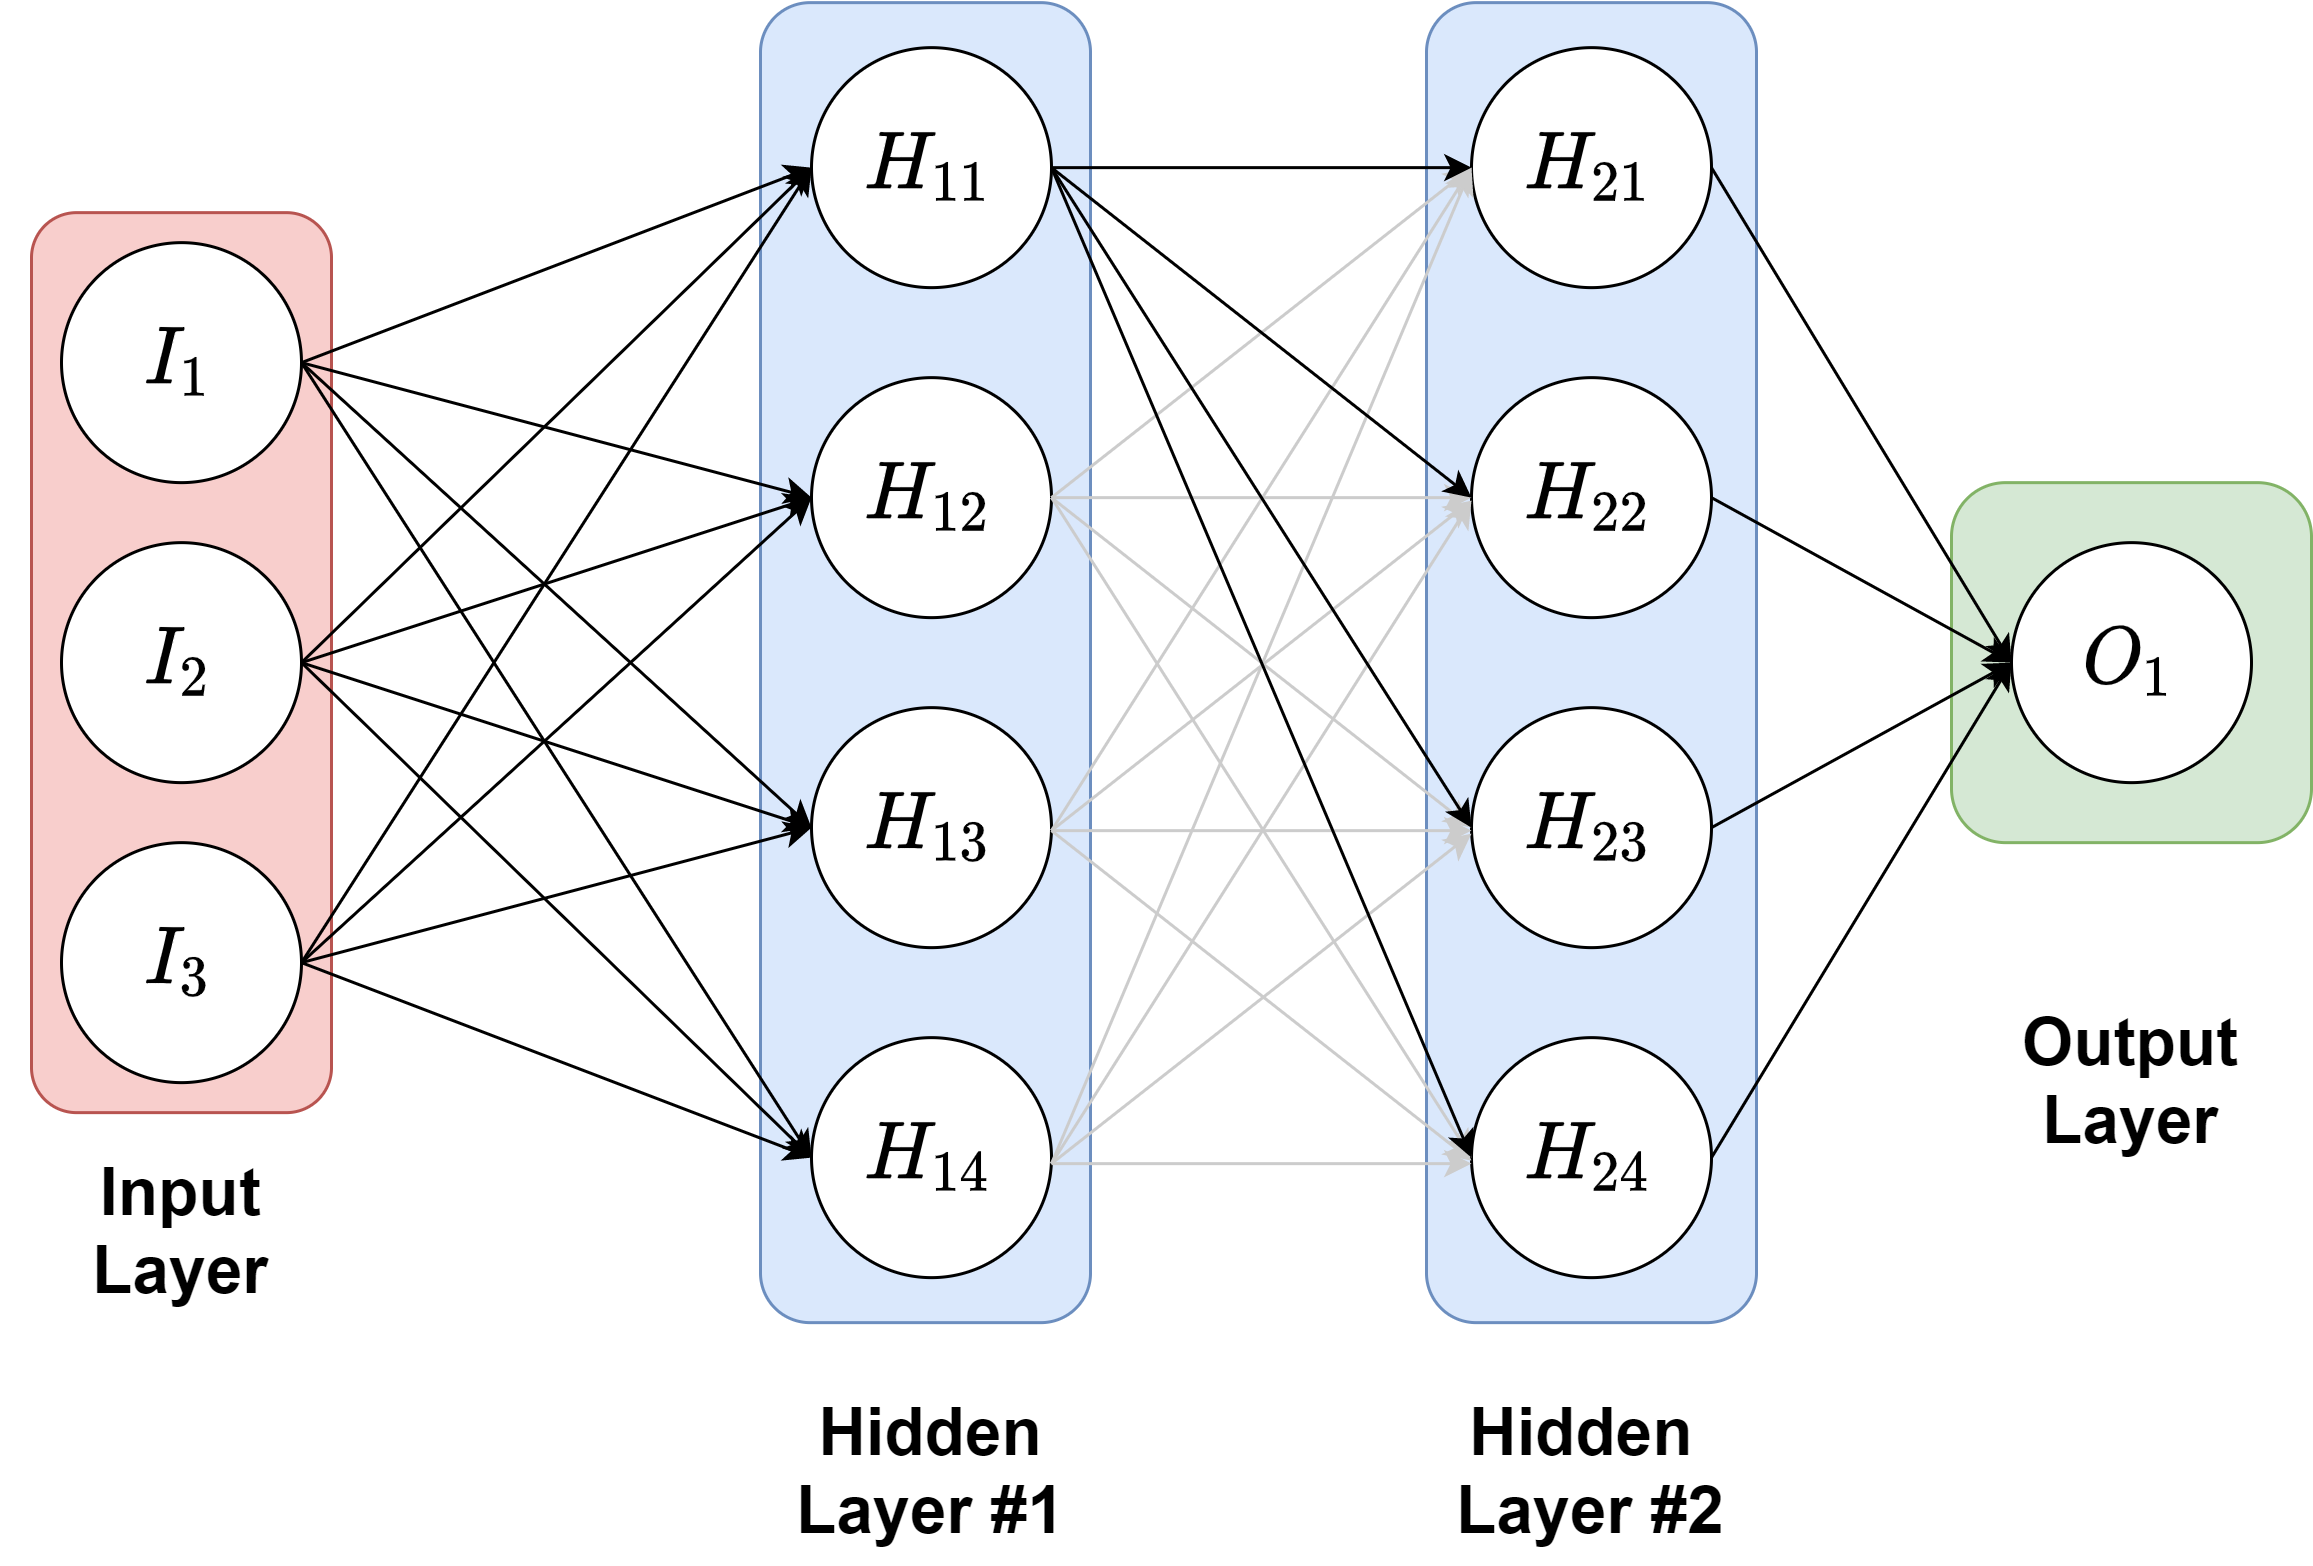
\includegraphics[width=0.65\textwidth]{Figures/Chp2_CNN/CNN_NN.png}
\caption{Artificial/Feedforward Neural Network with 2 hidden layers.}
\label{fig:ann_1}
\end{figure}

A loss function measures the quality of a particular set of parameters based on how well the induced scores agreed with the ground truth target in the training data. The loss function is dependent on training data and weights/ biases of the network. Since in Machine Learning, we take the training data as given and fixed, and weights as variables that we can control, we use back backpropagation to compute the gradients for the network parameters and perform a parameter update. Backpropagation is a way of computing gradients of expressions through the recursive application of the chain rule. The terminology of an N-layer neural network is such that we do not count the input layer. Therefore, a single-layer neural network describes a model with no hidden layers (input directly mapped to output). This same terminology will be followed for the CNN and RNN as well.

\section{Convolutional Neural Networks} \label{sec:CNN_CNN}
Convolution Neural Networks (ConvNets or CNN) are similar to ordinary Neural Networks in the sense that they are made up of learnable weights and biases. Each neuron will receive some inputs, multiplies them with weights (trainable parameters), and operates on it with a non-linear function. But the difference is that CNNs make an explicit assumption that input data follows a structured pattern to store the information (usually in the form of a uniform grid such as images, time-series events, etc.). This introduces certain properties in the architecture which helps in reducing the number of parameters in the network and makes the whole training process easier \parencite{goodfellow2016deep}.

A brief discussion on simple Feedforward Neural Networks is covered in Section \ref{ANN}. This will help in comparing and relating simple Neural Networks with CNNs.

\subsection{Architecture of the CNN based model} \label{sec:Arch_CNN}

There are three main types of layers present in CNN architecture: 
\begin{itemize}

\item \textbf{Convolutional layer(CONV)}: is used to compute the connection of each neuron with the local region of the input volume. It consists of a set of learnable filters/ kernels, as shown in Figure \ref{fig:CNN_FIG2A}. Each filter is small spatially as compared to the input image but slides across the whole length and width of the image and computes dot products between the entries of the filter and the input at any position creating a 2-D activation map/feature map giving the response of that filter at any position. The algorithm can learn appropriate filters that get activated for certain visual features, each filter looking for something new to learn.  When the 2-D activation map/ feature map is stacked together, they result in the output volume of a CONV layer. 

\begin{figure}
    \centering
    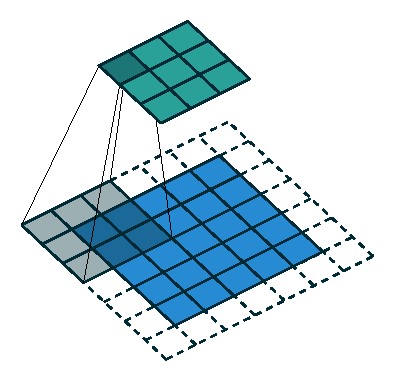
\includegraphics{Figures/Chp2_CNN/FIG2A.pdf}
    \caption{Convolution kernel visualization \parencite{dumoulin2016guide} (Blue = Input map, Cyan = Output map).}
    \label{fig:CNN_FIG2A}
\end{figure}

\item \textbf{Pooling layer (POOL)}: is in charge of downsampling the spatial dimension of the input. They are periodically inserted in-between CONV layers. The aim is to reduce the number of parameters in the network, thus helping in avoiding overfitting. The most popular form is a pooling layer with filters of size $2 \times 2$ applied with a stride of 2 (skipping a pixel), thus down-sampling every depth slice in the input by two along both width and height. It has two hyperparameters size and stride to control the volume of the output.

\item \textbf{Fully connected layer (FC)}: Neurons in these layers have a dense connection with all activations in the previous layers, similar to the architecture of regular Neural Networks. FC and CONV layers differ in the structure, as a CONV layer exhibits local connectivity and parameter sharing, but are identical in their functionality since both layers still compute the dot product between their weights and activations, followed by a non-linear activation function. The FC layer aims to balance the locality-context tradeoff. This layer can be thought of as relating all the features learned by the CONV layer to develop patterns that capture global trends.

\end{itemize}

The input to the DL network consists of uniformly placed spatial data where the neighboring pixels are related to each other. Grouping together the pixels that have similar attributes, through a convolutional filter is performed using a dense kernel as shown in Figure \ref{fig:CNN_FIG2A}. The traversal of the filter over the geometry results in a local measure of how likely two pixels are related to each other. In addition, a dilated filter is able to capture spatially distant relationships as shown in Figure \ref{subfig:CNN_FIG2B}.

\begin{figure}
    \centering
    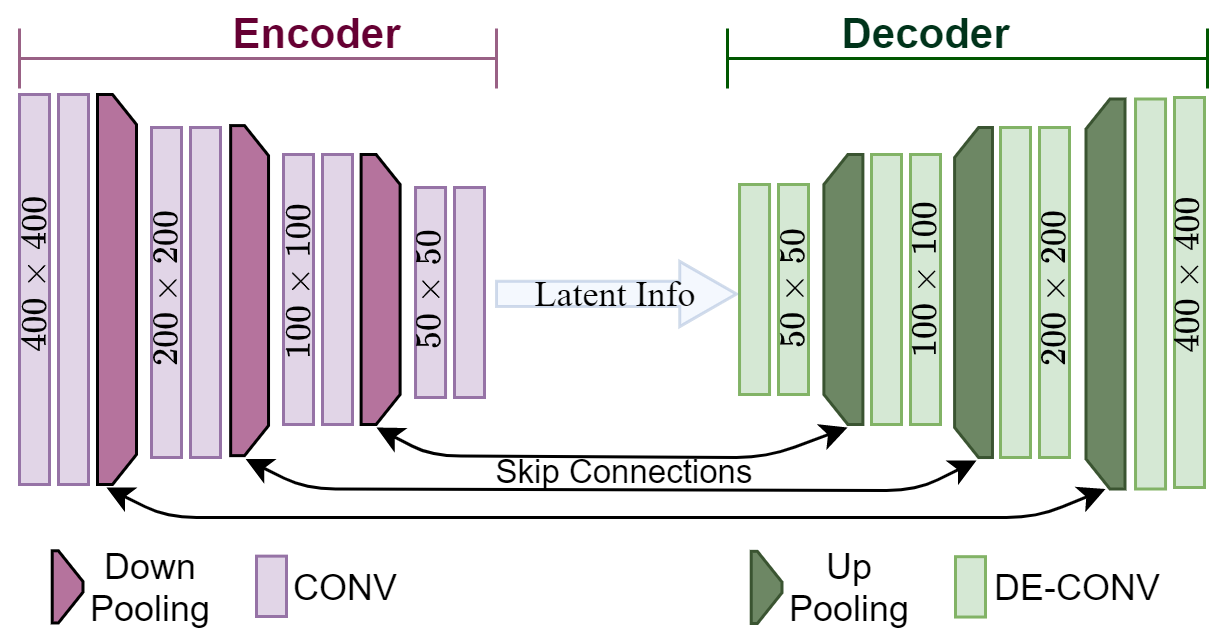
\includegraphics[width=0.95\textwidth]{Figures/Chp2_CNN/Network_arch.png}
    \caption{Encode-Decoder based Convolutional Neural Network Architecture}
    \label{fig:CNN_NN_arch}
\end{figure}

The DL model shown in Figure \ref{fig:CNN_NN_arch} and \ref{fig:cnn_nnarch_results} consists of a total of 32 layers with 16 trainable convolutional layers, 8 pooling/up-sampling layers and 8 dropout layers. Each block in the architecture consists of two sets of 3×3 convolution layers (including ReLU (Rectified Linear Unit \parencite{goodfellow2016deep}) and a batch-normalization layer \parencite{geron2019hands}), followed by a $2 \times 2$ max-pooling \parencite{goodfellow2016deep} (green arrow)/ up-sampling (blue arrow) layer with a stride of 2. This pattern is not followed for the last two convolutional layers due to a network design constraint, i.e. to fit the field distribution dimensionality. Each convolutional layer has a stride of 1. The network is trained using backpropagation with an aim to minimize the RMS error between the prediction and FEA field distribution. The limits on geometrical and excitation parameters mentioned in Section \ref{sec:CNN_DataCollection} are used to populate a design space using a Latin Hypercube. The dataset was then partitioned randomly into training, validation, and test sets. More information on the network and training dataset size can be seen in Table \ref{tab:cnn_nw_train_ds_features}. Although there are other techniques for partitioning the data, namely, cross-validation and bootstrap-based validation, the high computation cost associated with these techniques prohibited their usage in this case.

\begin{table}[]
\centering
\begin{tabular}{||c|c||c|c||}
\hline
\multicolumn{2}{|c|}{\textbf{Network Architecture}} & \multicolumn{2}{c|}{\textbf{Dataset}} \\ \hline \hline
Number of Layers              & 32                  & Training Dataset         & 30000      \\ \hline
Trainable Layers              & 16                  & Validation Dataset       & 10000      \\ \hline
Number of parameters          & 2.4 Million         & Test Dataset             & 5000       \\ \hline
\end{tabular}
\caption{Network and Training partition features.}
\label{tab:cnn_nw_train_ds_features}
\end{table}

\begin{figure}[h!]
    \centering
    \begin{subfigure}{0.45\textwidth}
        \centering
        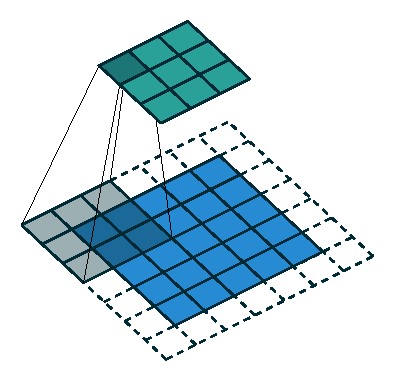
\includegraphics[width=\linewidth]{Figures/Chp2_CNN/FIG2A.pdf}
        \caption{Non-dilated Convolutional filter with padding.}
        \label{subfig:CNN_FIG2A}
    \end{subfigure}
    \begin{subfigure}{0.45\textwidth}
        \centering
        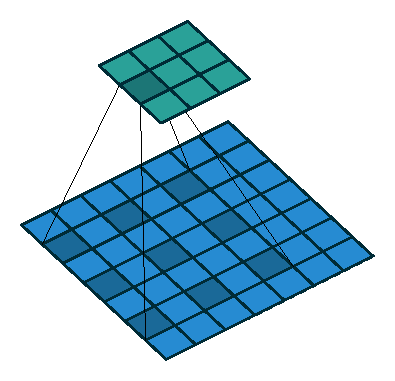
\includegraphics[width=\linewidth]{Figures/Chp2_CNN/FIG2B.pdf}
        \caption{Dilated filter with dilation rate of 1.}
        \label{subfig:CNN_FIG2B}
    \end{subfigure}
    \caption{Different types of kernel for a Convolutional layer in a CNN \parencite{dumoulin2016guide} (Blue = Input map, Cyan = Output map)}
\end{figure}

\subsection{Working of the DL model}\label{sec:Work_CNN}
The architecture of such a network resembles that for image segmentation purposes with the focus on dense regression instead of classification \parencite{badrinarayanan2017segnet}.
The network architecture can be divided into two parts: encoder and decoder, as seen in Figure \ref{fig:CNN_NN_arch}.  The encoder section tries to extract spatially related features from the input. This involves creating a bottleneck layer to compress out the most useful information from a high dimensional input, known as `latent representation'. This information is then used by the decoder section to semantically project the discriminative features learned by the encoder onto the original input space to predict the field solution.  For the network to train successfully, it must have sufficient capacity to satisfactorily capture the complexity of the problem \parencite{ghorbanian2017computer}. This capability is achieved by choosing an appropriate value for the number of layers, kernel size, number of kernels, and proper parameters for regularization. 
Model selection is usually performed by investigating a set of candidate models and choosing the one which gives the best balance between model fit and complexity. Random search and grid search are two of the common ways to arrive at optimal values of these hyperparameters \parencite{geron2019hands}. A total of 35 networks with different configurations were trained in the process of model selection. It is observed that the number of layers and the number of kernels/filters in a layer play an important role in the model performance. However, the most significant improvement is achieved by adding dilated filters, shown in Figure \ref{subfig:CNN_FIG2B}. This is a significant feature since the performance of the network improved not due to the addition of neurons but by changing the behavior of the constituent’s filters. A comparison is shown in Figure \ref{fig:cnn_training_results}, where a network with a kernel size of 5, number of kernels/filters in a convolutional layers (K) = 64, skip connections (shown in Figure \ref{fig:CNN_NN_arch} and \ref{fig:cnn_nnarch_results} (b)) and alternate dilated layers in the encoder outperforms other networks. The normalized RMS error in prediction over the validation shows an improvement for a network with dilation over the same network architecture with non-dilated (dense) kernels. The pattern is consistent for all three problems, with a similar accuracy level achieved for networks with K=32 and K=64 for the coil problem, as is shown in Figure \ref{fig:cnn_training_results} (a), (b) and (c). 

To gain intuition, we can think that the magnetic field at a point can be affected by regions far away from it (the source of excitation). The presence of dilation enables spatially far relations to be captured without increasing the kernel size. This is important for maintaining the locality-context trade-off of the network.

\begin{figure}[h!]
    \centering
    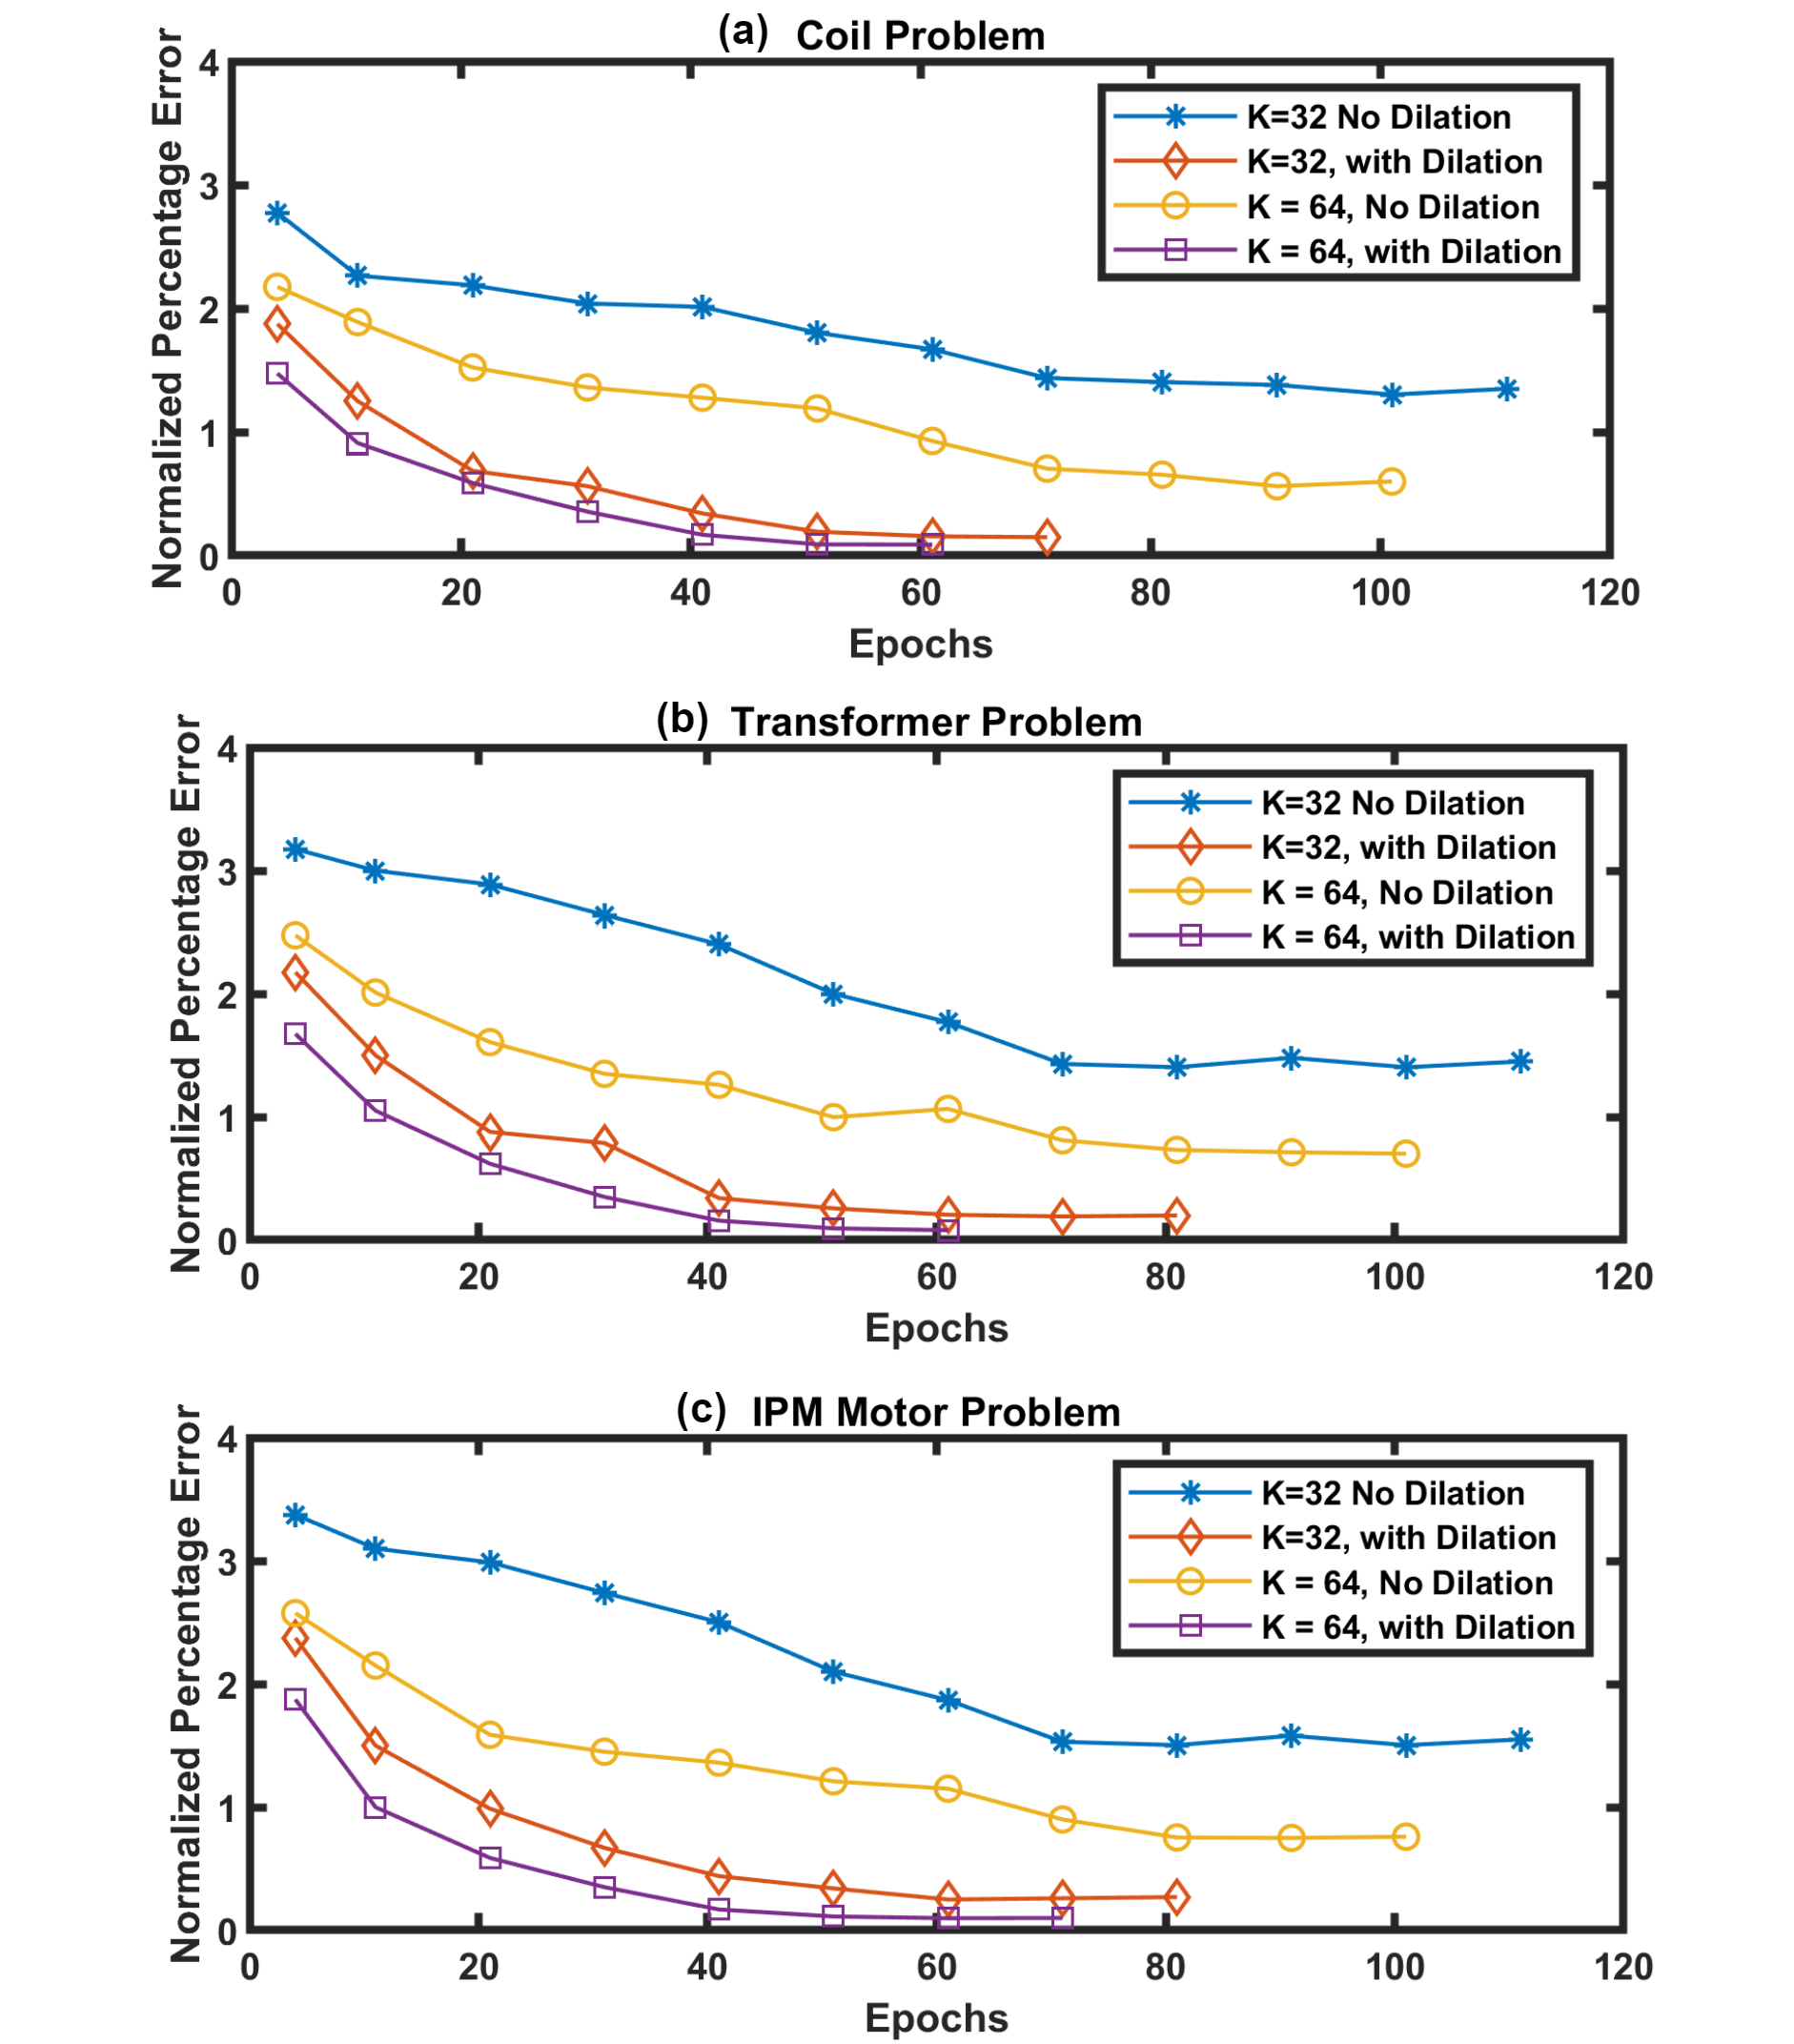
\includegraphics[width=\textwidth]{Figures/Chp2_CNN/Training_results3.png}
    \caption{Training curve with Normalized Prediction Error (calculated over validation dataset).}
    \label{fig:cnn_training_results}
\end{figure}

\section{Results \& Performance} \label{sec:results_CNN}

\begin{figure}[h!]
    \centering
    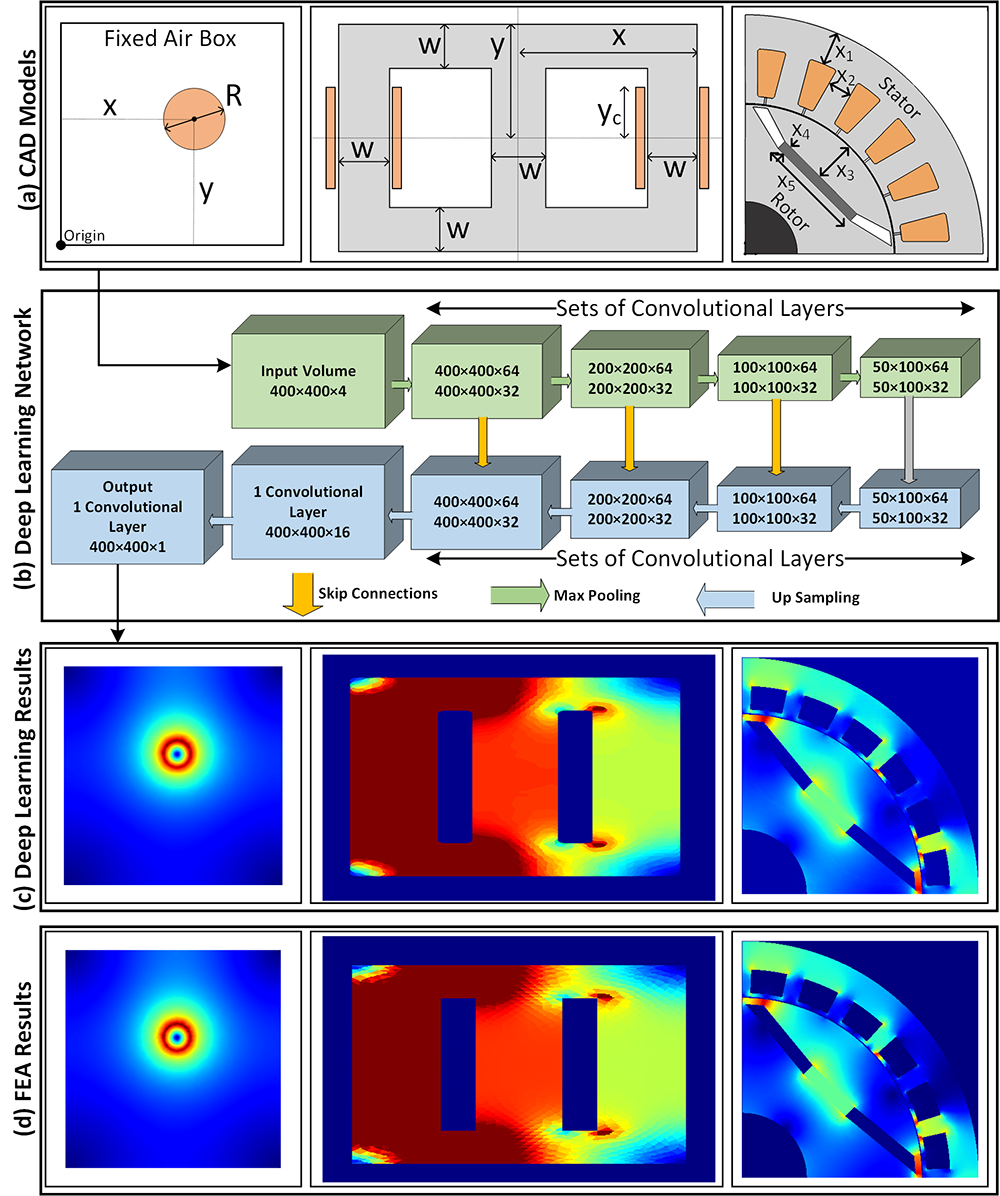
\includegraphics[width=\textwidth]{Figures/Chp2_CNN/NNArch_Results.png}
    \caption{(a) Problem definition, (b) Deep network architecture, (c) field predictions, (d) FEA results.}
    \label{fig:cnn_nnarch_results}
\end{figure}

Figure \ref{fig:cnn_nnarch_results} (c) shows the predicted magnetic field distribution in a coil, transformer and an IPM motor. The normalized mean squared error between the ground truth and the prediction lies in the range of 0.1\% - 1\% per node/pixel. The error distribution for an IPM motor can be observed in Figure \ref{fig:cnn_error_dist} and is highest around the corners, specifically in the carrier region of the rotor (boxed in black) and in the section of back iron (circled red). This was expected since a structured grid dense enough to capture these minute details will be computationally too expensive for this exploratory work. Although material exhibiting non-linear relations was included in the study, the performance of the network will deteriorate if the excitation is far different from that used for generating the dataset. 

\begin{figure}[h!]
    \centering
    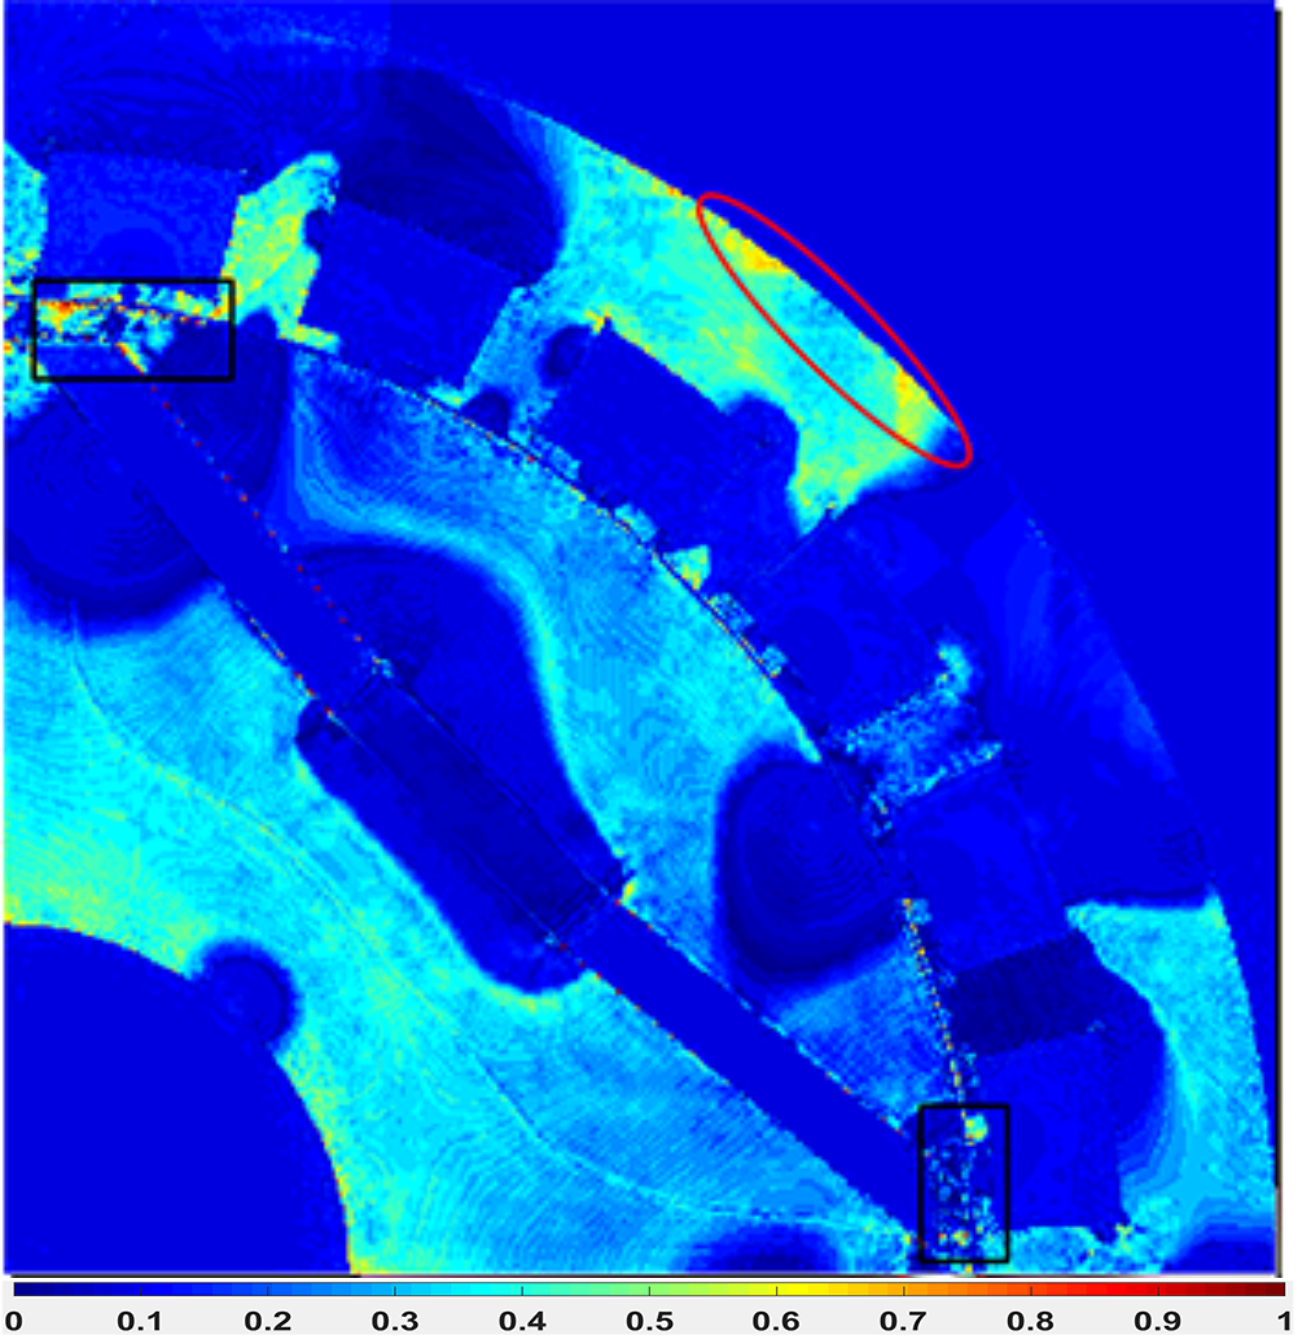
\includegraphics[width=0.65\textwidth]{Figures/Chp2_CNN/error_cnn_predVsTarget.png}
    \caption{Error (Ground Truth - Prediction) distribution.}
    \label{fig:cnn_error_dist}
\end{figure}

The network was trained on an NVIDIA 1080 Ti and took around 10 minutes per epoch with a batch size of 16. Convergence is achieved in around 60 - 100 epochs (depending on the network configuration, as shown in Figure \ref{fig:cnn_training_results}), resulting in a total run time of 12 – 15 hours. The prediction time is in the range of 2-3 seconds for 100 geometries at a time (batch size). The time required to analyze multiple geometries is memory-bound rather than compute-bound, i.e. it is possible to parallelize the training and inference to thousands of samples if the memory requirements are satisfied.

\section{Uncertainty Prediction}

The DL trained in this work and some other works \parencite{tang2017study} employ supervised training and the prediction accuracy depends on how close the input is to the training data. A geometry that is significantly different from the ones in the training dataset will produce substantial errors. To be able to rely on such a predictor (trained in a supervised manner), we need to provide a measure of uncertainty in the results. This knowledge is essential to quantify the confidence one can have in the results. One way to achieve this is by extending the DL model by introducing a probabilistic component in the neuron weights.
The technique is based on quantifying uncertainty known as Monte- Carlo (MC) dropout \parencite{gal2016dropout}. Monte Carlo integration gained popularity during the Manhattan Project. Due to its effectiveness, it was included in the top 10 algorithms of $20^{th}$ century \parencite{Metropolis}. Instead of generating a system of the equations to describe a complex problem, we can simulate it multiple times and average out the quantity we are interested in.

\subsection{Uncertainty Maps}

Uncertainty maps are images that indicate the model's uncertainty for a given pixel classification. It may be tempting to interpret the values from the final softmax layer of a CNN as confidence scores, but we must be careful as work on Adversarial Networks have shown that minute perturbations to a real image can change the softmax output to arbitrary values \parencite{goodfellow2014explaining}. This can make the network predict wrong results with high confidence. A network will try to predict even in cases where the input data itself might be irrelevant. This is especially important when dealing with images that were not present during training. \parencite{gal2016dropout} showed how we can use dropout in a deep CNN to get uncertainty information from a model’s predictions. Instead of having fixed weights, each weight is drawn from a distribution.

Quantifying the uncertainty in the network’s prediction would allow us to find regions in an image for which the network is unsure of its prediction. Furthermore, segmentation based on an uncertainty threshold value can sort out the pixels over which the model is confident in the prediction, thus providing us with a partial but highly accurate solution.

\subsection{Theory} \label{section:CNN_MC_theory}

Dropout \parencite{srivastava2014dropout} was introduced as a regularization technique with an aim to check the bias-variance tradeoff of the network. The technique involves a parameter ($p$), which determines the probability of dropping out any neuron from the network for an iteration during the training on the dataset ($X,Y$). Thus, training a neural network with dropout is equivalent to training a collection of $2^K$ thinned networks with extensive weight ($W$) sharing, but a single network approximates the average output at test time, through a weight averaging technique \parencite{badrinarayanan2015segnet}. Thus, assuming a point estimate for weights. On the other hand, dropout variational inference is a practical approach for approximate inference in large and complex models \parencite{kendall2015bayesian}. 

Even with a small number of parameters, inferring the model posterior distribution $(p(W \vert X,Y))$ in a Bayesian NN is a difficult task, with the variational inference being a popular approach to approximate the posterior distribution. This is done by minimizing the Kullback-Leibler divergence from the true posterior $(p(W \vert X,Y))$. However, this approach can be very computationally expensive, almost doubling the number of model parameters \parencite{blundell2015weight}. On the other hand, it has been shown that dropout can be cast as approximate Bayesian inference in Gaussian processes. This means that uncertainty information can be extracted from models without requiring additional parameters. Usually, training a neural network with dropout can be seen as training a collection of $2^K$ thinned networks with extensive weight sharing, but a single network approximates the average output at test time. Thus assuming a point estimate for weights. 

Instead, performing dropout during the test phase can be viewed as performing Monte Carlo sampling from the posterior distribution over the various dropout models. By applying dropout to all the weight layers, we are essentially drawing weight from a Bernoulli distribution. This technique has been utilized in order to produce uncertainty maps as a measure of prediction uncertainty. This work is in line with Bayesian SegNet \parencite{kendall2015bayesian}. However, this work extends this information to more than a visualization tool and relates uncertainty information and segmentation accuracy. 

We are interested in finding the posterior distribution over the convolutional weights, $W$ given the observed training data: input ($X$) and target ($Y$).
    \begin{gather*} 
    p(W\vert X,Y)
    \end{gather*}

Unfortunately, this posterior distribution is not tractable.
  \begin{gather*} 
    p(W\vert X,Y) = \frac{p(Y\vert X,W)\times p(W)}{P(X)}
    \end{gather*}
The evidence term : $p(X) = \int p(X, W) \times p(W) dW$, is very difficult to compute. We need to approximate the distribution of the weights (W). We can use Variational Inference (VI) to approximate it. Here we learn a distribution q(W), by minimizing the Kullback-Leibler divergence between this approximate distribution \& the true posterior:

\begin{gather*} 
    KL \, (q(W) \enspace \vert \vert \enspace p \, (W\vert X,Y)).
\end{gather*}
    
Since dropout is seen as an approximation to a Bayesian Network, the uncertainty in the weights induces a prediction uncertainty.
\begin{gather*} 
    p(y\vert x,X,Y) =  \int p(y\vert x,W) \times p(W \vert X, Y) dW
    \end{gather*}

Since the true posterior is intractable, we approximate the posterior using Monte Carlo integration:
\begin{gather*} 
    p(y\vert x,X,Y) =  \int p(y\vert x,W) \times q(W) dW
    \end{gather*}

How to implement this? With Dropout, a unit is present with a probability `$p$', and at testing the unit is always present and the weights are multiplied by `$p$'. In practice, we can sample from the distribution by running several forward passes through the network.  Dropout can be cast as approximate Bayesian inference over the network’s weights. This imposes a Bernoulli distribution over the CNN filter’s weights.

\begin{comment}

% Another version
This inference is made by training a model with dropout before every weight layer, and by also performing dropout at test time to sample from the approximate posterior (stochastic forward passes, referred to as MC dropout sampling). So, the distribution over the network weights (W), given the observed training data: input (X), and labels (Y), is given as:
\begin{align}
    p(W|X, Y)
\end{align}

Unfortunately, this posterior distribution is not tractable, due to the evidence (P(X)) term.

\begin{align}
    p(W|X, Y) = \frac{p(Y|X, W) \times p(W)}{p(X)}
\end{align}

By applying dropout to all the weight layers, we are essentially drawing weight from a Bernoulli distribution [16]. Instead of having fixed weights, each weight is drawn from some distribution. Sampling from a distribution introduces uncertainty in the prediction.

\begin{align}
    p(y|x, X, Y) = \int p(y,x,W) \times p(W|X, Y)dW
\end{align}

Since the true posterior is intractable, we approximate the posterior using MC integration:

\begin{align}
    p(y|x, X, Y) = \int p(y,x,W) \times q(W) dW
\end{align}

More formally, dropout can be cast as approximate Bayesian inference, thereby extracting the uncertainty information without requiring additional parameters. This is implemented as follows: With dropout, a unit is present with a probability ‘$p$. We can sample from the distribution by running several forward passes through the network. 
A mathematical study on the theory of MC dropout can be found in [16][18].
\end{comment}

\section{Bayesian Network - Results}

\begin{figure}[h!]
    \centering
    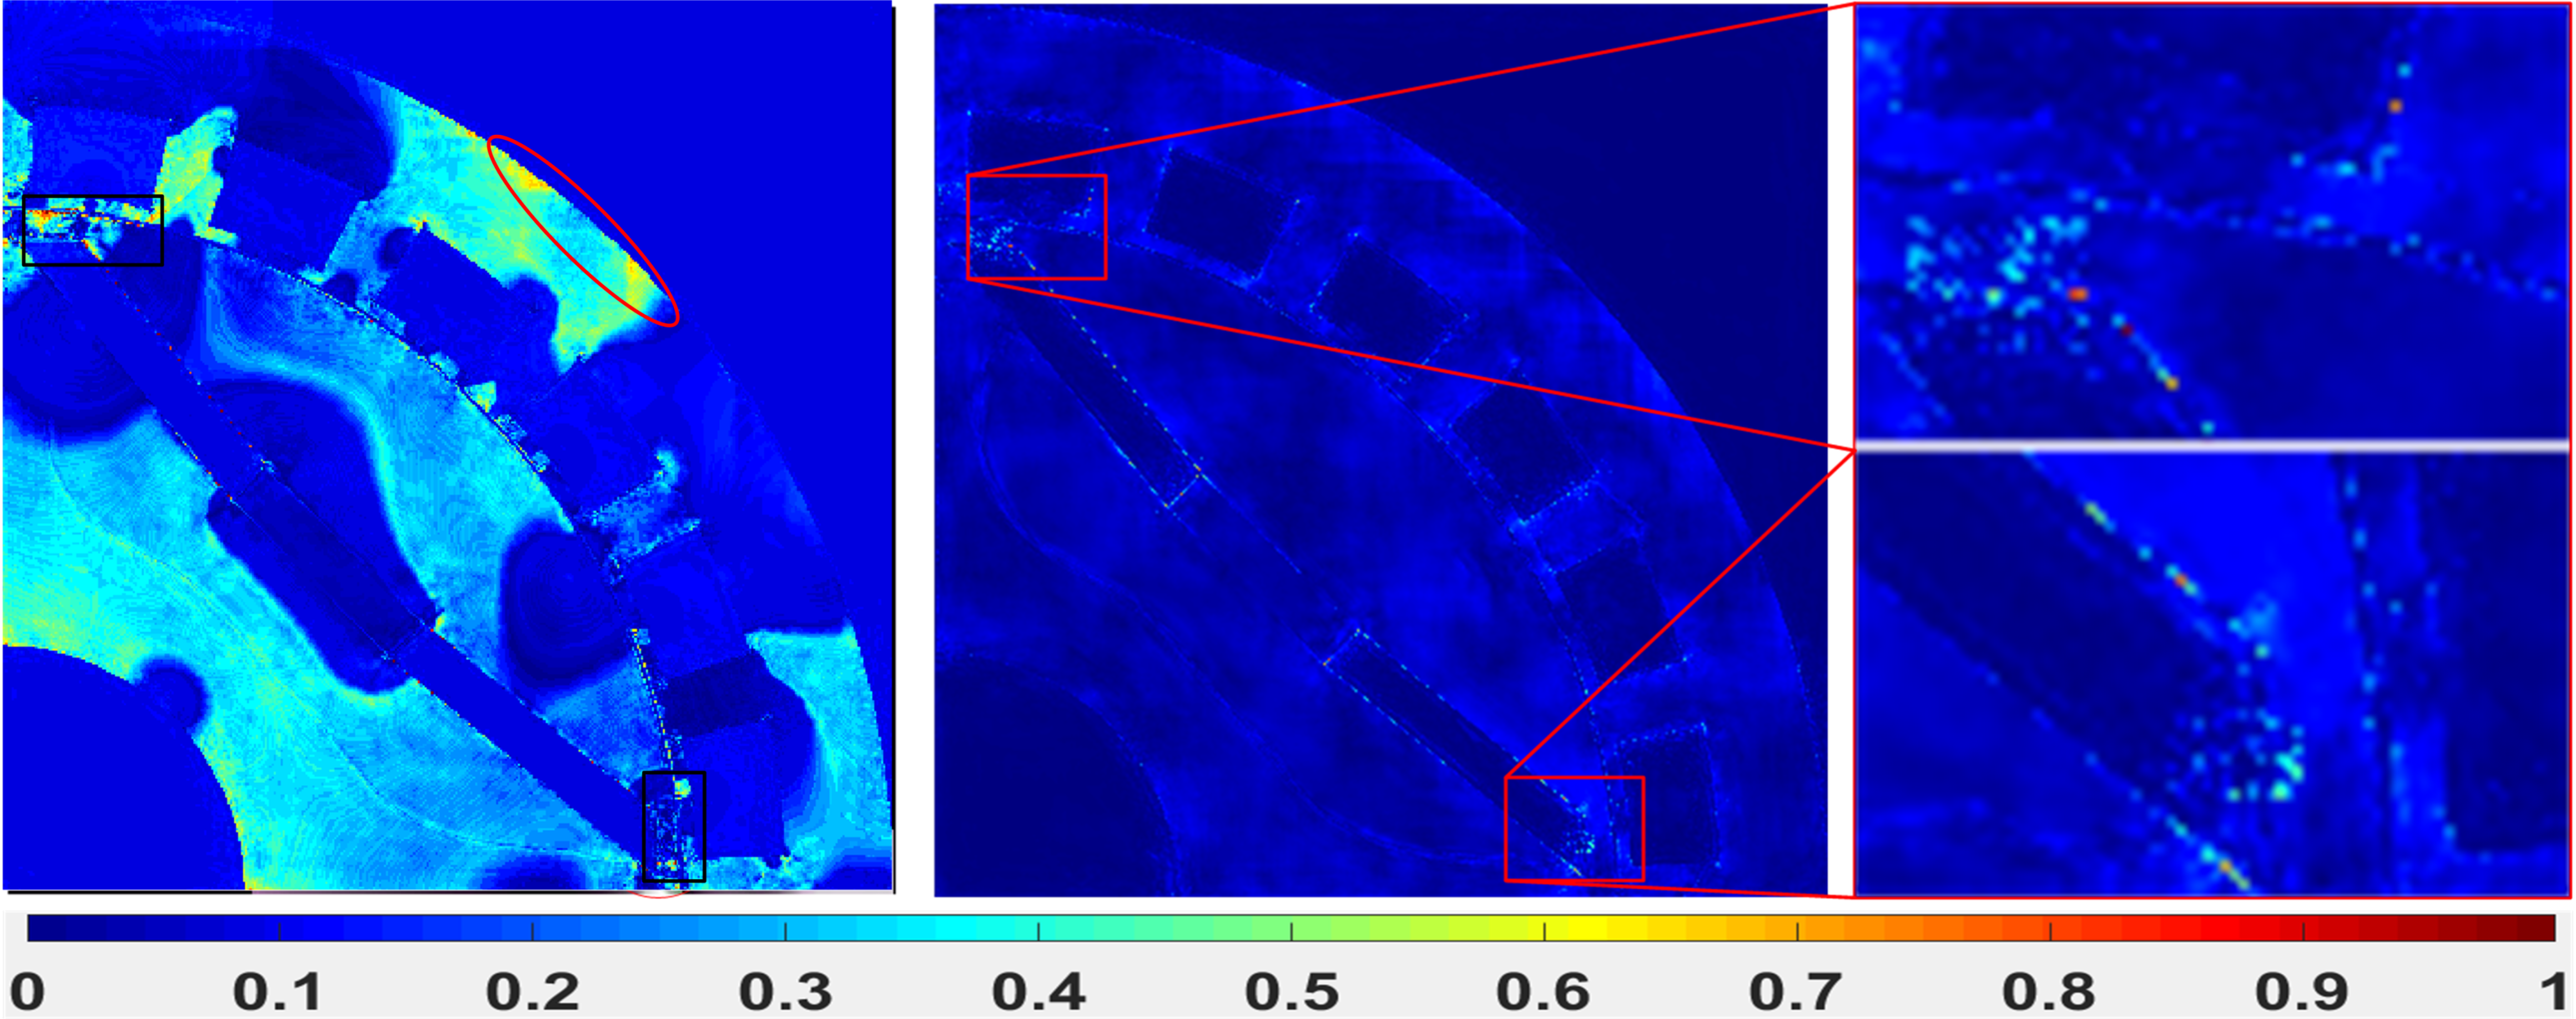
\includegraphics[width=\textwidth]{Figures/Chp2_CNN/Fig 4_updated5.png}
    \caption{(a) Error distribution, (b) Normalized uncertainty map from Bayesian Inference, (c) Region of uncertainty map with high uncertainty.}
    \label{fig:cnn_error_analysis}
\end{figure}

Using Monte Carlo (MC) dropout \parencite{gal2016dropout}, uncertainty maps are computed for all three CNNs by retrieving 10 Monte Carlo samples from the networks and then calculating the standard deviation over the softmax outputs of the samples. In this Chapter, if not stated otherwise, the uncertainty maps are displaying the mean standard deviation over all the classes. Besides the uncertainty maps, Monte Carlo sampling has also been shown to be valuable to increase classification accuracy \parencite{kendall2015bayesian}, as it has been shown to outperform the standard weight averaging technique. A qualitative measure can also be extracted by generating uncertainty maps. A normalized uncertainty map through such implementation is shown in Figure \ref{fig:cnn_error_analysis}(b), with regions of high uncertainty highlighted and expanded in Figure \ref{fig:cnn_error_analysis}(c). Figure \ref{fig:cnn_error_analysis}(a) shows the error distribution between the prediction and ground truth. It can be seen that the standard deviation of the Monte Carlo samples (Figure \ref{fig:cnn_error_analysis}(b)), is related to classification accuracy. A high value of uncertainty is an indication to not rely on the results and perhaps employ the generalized conventional solvers (FEA, FDM, etc.).  Out of the three regions of high error (circled in Figure \ref{fig:cnn_error_analysis} (a)), the Bayesian approach could relate two (black box in Figure \ref{fig:cnn_error_analysis}(a)) with high uncertainty. The uncertainty maps are computed by retrieving 10 MC samples from the network and calculating the standard deviation over the samples. Besides the uncertainty maps, MC sampling improved the accuracy (normalized mean squared error) by around 10\%.

\section{Conclusion}
By learning the field distribution from the FEA software, our model efficiently approximated the distribution. This enables us to generate the field distribution for new geometries at lower computational costs, with the added advantage of parallelizability over GPUs. A probabilistic way of analyzing the prediction without the ground truth is also presented. Thus, providing the decision-making capacity to either use the estimated field for post-processing or revert to other numerical solvers.
Although a structured CNN is not the ideal architecture to handle an unstructured mesh as is employed in FEA, the DL field estimator model can function as an initial guess for the FEA solver. With recent advancements in Graph Convolutional networks, which are more suited to handle unstructured meshes, we hope to extend this work to come up with an improved predictor in the future. Another bottleneck is the amount of simulated (big) data required for training a deep network. An approach involving semi-supervised or unsupervised learning can offer an exciting path with less dependency on labeled data. Nonetheless, this work can provide guidelines for selecting a suitable network design for future work in this field. 


 Crucially, the proposed approach shows good accuracy in magnetic field prediction and can take advantage of GPUs for fast training. Through this chapter, essential guidelines for setting up deep networks are established, the result/inference is improved by Bayesian techniques and the confidence levels of predictions are evaluated appropriately. 
 
 The work presented in this chapter serves as foundation for exploring the usage of DL models for other computationally expensive tasks such as performance maps, namely efficiency and power factor maps. These will be discussed next in Chapter \ref{chapter:3_RNN}.
 
 
 \begin{comment}
 
 
 The model from here on will be referred to as a DL field estimator. In this work, the DL network is trained in a supervised fashion with inputs consisting of information regarding design geometry, excitation, and material properties. The ground truth consists of magnetic field distributions over the input domains, simulated from traditional FEA solvers.

However, it is comparatively much slower and can benefit from a deep learning model which is computationally cheaper. In the next section, few deep learning models to replicate the performance of FEM are discussed.

Further, we wish to use this network as a generative model to predict the performance of a design based on its understanding of the physics involved in the whole process.


\end{comment}
 